\subsection{Discussion of the closures for non-inertial spherical droplets}

The closure terms appearing in the above equation are the results of the ensemble average operator $\avg{\ldots}$. 
In all rigor, we cannot compute theoretically such an average since it necessitate to know the distribution $P(\FF)$ and the exact expression of the local terms indicated by the notation $(\ldots)^0$. 
In the same spirit as in \citet{batchelor1972sedimentation,hinch1977averaged} and \citet{zhang1994averaged} we demonstrate here that it is therefore necessary reformulate the closure term to remove the ensemble average procedure. 
We demonstrated in \ref{ap:Closure_problem} that any ensemble averaged quantities can be reformulated as an integral of what we call \textit{conditionally averaged quantities}. 
The expression obtained are then consistent with \citet{batchelor1972sedimentation,hinch1977averaged} and \citet{zhang1994averaged} but somewhat more general. 
In a second step we demonstrate how to derive what we call the \textit{conditionally averaged equations} that are needed to obtain the \textit{conditionally averaged quantities}. 
Again our derivation is directly inspired by the cited author, but the approach is generalized in many ways. 
For instance, in dilute and low Reynolds number assumption these equations correspond to the classic problem of the disturbance field generated by a translating droplet in an otherwise quiescent liquid flow. 
The real interest behind this demonstration is that it is kept general and offers many possibilities for extension of the model.
While more complicated considerations cannot be usually solved theoretically, these general formulations extend our current understanding of the closure problem. 

Consequently the closure presented in this section are based on the singularity solution of an isolated droplet in linear flow. 
For illustrating purposes we displayed on \ref{fig:flowlines} the flows line of such a solution both uniform flow as well as linear flows. 
\begin{figure}[h!]
    \centering
    \begin{tikzpicture}
        % \node (img3) at (0.6\textwidth,0) {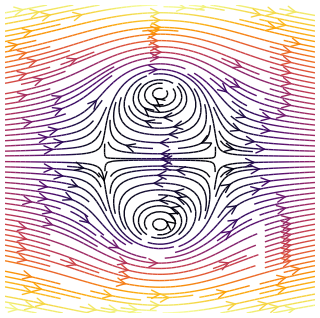
\includegraphics[width=0.3\textwidth,angle=270]{image/Rising_def_Stokes.png}};
        \node (img2) at (0.3\textwidth,0) {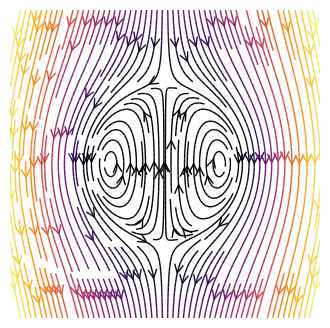
\includegraphics[width=0.3\textwidth]{image/Rising_Stokes.png}};
        % \draw (0.45\textwidth,0)node{$\rightarrow$};
        % \draw (0.45\textwidth,0.4cm)node{$\bm\Gamma_\alpha\cdot \textbf{r}$};
        \node (img1) at (0.0\textwidth,0) {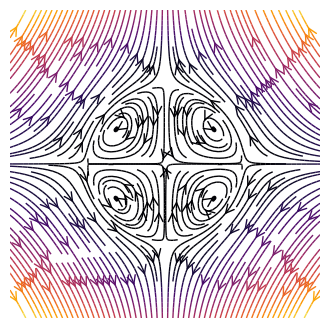
\includegraphics[width=0.3\textwidth]{image/Shear_Stokes.png}};
        % \draw (img3.south)node{(c)};
        \draw (img2.south)node{(b)};
        \draw (img1.south)node{(a)};
    \end{tikzpicture}
    \caption{Examples of steady state flow lines plots of an isolated droplet immersed into a viscous fluid. 
    (a) Rising sphere in uniform stokes flow. 
    (b) Fixed droplet in a pure extensional.
    (analytical solution in \ref{ap:Closure_problem})}
    % (c) Deformed droplet in rising motion (analytical solution of \citet{taylor1964deformation}). }
    \label{fig:flowlines}
\end{figure}

\subsubsection{Moment of force traction}

For purpose of understanding, we have re-derived in \ref{ap:Closure_problem}, the momentum exchange term present in of \ref{eq:dt_hybrid_rhou_f} for dilute suspension of spherical droplets. 
% Specifically, we consider an isolated spherical non-rotating droplet of viscosity $\lambda \mu_f$ immersed in an arbitrary linear flow. 
% Most of the term present in \ref{eq:dt_hybrid_rhou_f} are discussed in\ref{ap:two-fluid_model}, thus let focus on the three exchangek terms.  
It is found that the first three moment of the hydrodynamic forces are related to the mean fluid phase velocity field as, 
\begin{align}
    \label{eq:zeroth_mom}
    \pSavg{\bm{\sigma}_f^0\cdot \textbf{n}_d} &= 
    \phi_d \div\bm\sigma_f
    + \frac{3\phi_d\mu_f}{2 a^2} 
    \left(\frac{3\lambda+2}{\lambda+1}\right) \textbf{u}_{f p} 
    + \frac{3\phi_d\mu_f}{4} \left(\frac{\lambda}{\lambda+1}\right)\grad^2\textbf{u}_f\\
    \label{eq:first_mom}
    \pavg{\intS{\textbf{r}\bm{\sigma}_f^0 \cdot \textbf{n}_d}} 
    &= 
    \phi_d \bm\sigma_f + 
    \frac{3}{5}\mu_f \phi_d \left(\frac{2+5\lambda}{1+\lambda}\right)
    \textbf{E}_f
    \\
    \label{eq:second_mom}
        \pavg{\intS{(\bm{\sigma}_f^0 \cdot \textbf{n}_d)_ir_kr_l}} &=
        % \phi_d  \frac{a^2}{5} 3 [(\div \bm\sigma_f)\bm\delta]^\text{sym}
        + \frac{3\mu_f\phi_d}{2}\left(\frac{\lambda}{\lambda+1}\right)(\textbf{u}_{fp})_i\delta_{kl}\\
        &+ \frac{3\mu_f\phi_d}{5}\left(\frac{1}{\lambda+1}\right)((\textbf{u}_{fp})_i\delta_{kl}+ (\textbf{u}_{fp})_k\delta_{il}+(\textbf{u}_{fp})_l\delta_{ki})\nonumber
\end{align}
where $\textbf{u}_{fp} = \textbf{u}_f - \textbf{u}_p$ and $\textbf{E}_f = \frac{1}{2}\left[\grad \textbf{u}_f + (\grad \textbf{u}_f)^\dagger\right]$. 
Note that at first order in $\phi_d$, $\phi_d\textbf{u}_f =\phi_d\textbf{u} - \phi_d^2 \textbf{u}_d = \phi_d\textbf{u}$, so one can either use $\textbf{u}_f$ or $\textbf{u}$ in the above definition. 
The term $\pSavg{\bm{\sigma}_f^0 \cdot \textbf{n}_d}$ represents the total components of the interphase drag force.
Specifically, the first term is the mean fluid phase stress $\bm\sigma_f$ (including buoyancy forces), the second term is the Hadamard-Rybczynski force and the last is the Faxen contribution \citep{kim2013microhydrodynamics}. 
Likewise, $\pSavg{\textbf{r}\bm{\sigma}_f^0 \cdot \textbf{n}_d}$ is the averaged first moment of the surface force traction, which includes the mean fluid phase stress. 
This tensor is responsible for the well-known Einstein correction to the viscosity (see next section), but here it is adapted to spherical droplets instead of spherical solid particles \citep{rallison1978note}. 
% Therefore, this term is of upmost importance in the averaged momentum equations and is non-negligible in most of the flow conditions, if not all of them.
The second moment of the force traction is made of three contribution, the first one is related to the divergence of the mean fluid phase stress, see \ref{eq:second_mom_general}. 
However, this contribution is negligible at $\mathcal{O}(\phi_d)$ \citep{jackson1997locally} and therefor not shown in \ref{eq:second_mom}.  
The second contribution is proportional to the relative velocity $\textbf{u}_{fp}$.
This was firstly discovered by \citet{nozieres1987local} based on phenomenological arguments and by \citet{lhuillier1992volume} based on theoretical ground, both for spherical solid particles. 
According to the cited author this term induce a coupling between relative motion and convection. 
The second moment of the hydrodynamic forces is non-negligible at first order in $\phi_d$, in agreement with \citep{jackson1997locally,zhang1997momentum}. 
Thus, the zeroth, first and second moment of the drag are non-negligible in the Stokes regime and at $\mathcal(\phi_d)$. 
In \citet{zhang1997momentum} they even stipulated that the third order moment of the force traction is not necessarily negligible at $\mathcal{O}(\phi_d)$ when considering non-spherical particles in stokes flows. 
Consequently, out of the stokes and dilute hypothesis, the zeroth, first and third moments of surface traction are non-negligible and are primordial in the modeling of the fluid phase momentum equations. 
% It is surprising that most of the study only concentrate on the modeling of \ref{eq:zeroth_mom}. 

\subsubsection{Pseudo turbulent stress}

Another contribution to the stress is the pseudo-turbulent tensor $\avg{\chi_f \textbf{u}_f'\textbf{u}_f'}$. 
Note that in stokes regime this term is more likely to be negligible, nevertheless it is still interesting to provide its closure as it gives bases for possible finite inertia model. 
In \ref{ap:Closure_problem} we compute the first order correction to this stress, it yields, 
\begin{multline}
    \avg{\chi_f \rho_f \textbf{u}_f' \textbf{u}_f'}
    =
    \frac{\phi_d a^2 \rho_f}{105 (\lambda +1)^2 }\left[
        (129\lambda^2+108\lambda+24)\textbf{E}_f\cdot \textbf{E}_f
        + (20\lambda^2 +20\lambda + 6)
        (\textbf{E}_f : \textbf{E}_f)\bm\delta
    \right]\\
    + C_1(\phi) [\textbf{u}_{fp} \textbf{u}_{fp}
    + \pavg{\textbf{u}_\alpha'\textbf{u}_\alpha'} ]
    + C_2(\phi) [\textbf{u}_{fp}\cdot \textbf{u}_{fp} + 2 n_p k_p]\bm\delta
    \label{eq:Reynolds_stress}
\end{multline}
Where $C_1$ and $C_2$ are unknown constant.
Indeed, the disturbance fields of a droplet in translation is proportional to $r^{-1}$ thus the computation of the integral of $\avg{\chi_f \rho_f \textbf{u}_f' \textbf{u}_f'}$ diverges. 
However, since the disturbance field of a droplet in translation is proportional to the relative velocity $\textbf{u}_{fp}$ the functional form of this tensor cannot be otherwise that proportional to $\textbf{u}_{fp} \textbf{u}_{fp}$ and $(\textbf{u}_{fp}\cdot \textbf{u}_{fp})\bm\delta$.
Additionally, for spheres in ordered immersed in a uniform flow we have $C_1(\phi) \sim \phi^{2/3}$ \citet{hill2001first}.
It is therefore reasonable to expect the same trend for random array since in the dilute regime both are supposed to be equivalent. 
Another example is that of a spherical bubble in relative motion with a potential flow, in which case the pseudo turbulent tensor also takes the form of the second line of \ref{eq:Reynolds_stress} (see equation (5.7) of \citet{zhang1994ensemble}). 
A droplet immersed in a linear flow also produce pseudo-turbulence. 
The contribution from the mean shear flow to the pseudo turbulent tensor is also derived in \ref{eq:Closure_problem} and reads as the first line of \ref{eq:Reynolds_stress}. 
In  \citet{raja2010inertial} they study theoretically the stress in a neutrally buoyant suspensions of droplets. 
In the dilute limit they compute the deviatoric part of $\avg{\chi_f \rho_f \textbf{u}_f' \textbf{u}_f'}$ based on the stokes flow solution. 
It is observed that the first term on the right-hand side of \ref{eq:Reynolds_stress} is consistent with equation (3.15) of \citet{raja2010inertial}.
Regarding the second term of \ref{eq:Reynolds_stress} it corresponds to the  isotropic contribution of the Reynolds stress.
This term seems new  


\subsubsection{The fluid phase equivalent stress}
% In this section we focus on the formulation of the averaged fluid phase equivalent stress tensor $\bm{\sigma}_f^\text{Re}$. 
For instance the stress appearing on the left hands side of the fluid phase momentum balance is of the form of \ref{eq:sigma_eq_def}. 
It is more convenient to express the equivalent stress as a Newtonian stress, plus a contribution arising due to the presence of the particles. 
Thus, we reformulate $\bm{\sigma}_f$ considering that $\phi_f \bm{\sigma}_f = - \phi_f p_f + 2 \phi_f \mu_f \textbf{e}_f$ where $2 \phi_f \bm{e}_f = \avg{\chi_f  (\grad \textbf{u}_f^0 + (\grad \textbf{u}_f^0)^T)}$. 
Additionally, we state that the fluid strain is equal to the bulk strain $2\textbf{e} = \grad \textbf{u}+ (\grad \textbf{u})^T$, minus the particle averaged strain, i.e. $\phi_f \mu_f \textbf{e}_f = \mu_f\textbf{e} - \mu_f \phi_d \textbf{e}_d$ which gives
\begin{equation*}
    \bm\sigma_f\phi_f =-\phi_f p_f \bm\delta + 2 \mu_f \textbf{e} -2\phi_d \mu_f \textbf{e}_d.
    \label{eq:def_sigma_f}
\end{equation*}
Under this form we clearly remark that for solid particle $\phi_d \textbf{e}_d = 0$ thus we recover equations (44) of \citet{jackson1997locally} which reads in our notation : $\bm\sigma_f\phi_f =-\phi_f p_f \bm\delta + 2 \mu_f \textbf{e}$. 
Upon developing $\phi_d \textbf{e}_d$ multipolar series using \ref{eq:f_exp}, the equivalent stress of the fluid phase can be reformulated as, 
\begin{multline}
    \bm{\sigma}^\text{eq}_f = 
    \phi_f p_f \bm\delta 
    - 2\mu_f \textbf{e} 
    +\avg{\rho_f\chi_f\textbf{u}_f'\textbf{u}_f'} 
    + 2 \mu_f \pOavg{\textbf{e}_d^0}
    - \pSavg{\textbf{r}\bm{\sigma}_f^0\cdot \textbf{n}_d}
    \\
    + \div \left[
        \frac{1}{2} \pSavg{\textbf{rr}\bm{\sigma}_f^0\cdot \textbf{n}_d}
        - 2 \mu_f\pOavg{ \textbf{re}_d^0 }
        + \ldots
    \right]
    \label{eq:sigma_eq_0}
\end{multline} 
It is worth noting that $\textbf{e} = \grad \textbf{u} + (\grad \textbf{u})^\dagger$. 

Nevertheless, the bulk velocity \textbf{u} is not part of our unknown instead we solve for $\textbf{u}_f$, $\textbf{u}_p$, $\textbf{P}_p$ and eventually the higher moments. 
Therefore, in all rigor we must write 
\begin{equation}
    \textbf{e}
    = 
    \grad \textbf{U} + (\grad \textbf{U})^\dagger
    - \grad (\div (n_p \textbf{P}_p))
    - (\grad \div (n_p \textbf{P}_p))^\dagger
    + \ldots
    \label{eq:rate_of_strain}
\end{equation}
where $\textbf{U} = \phi_f \textbf{u}_f + n_p v_p \textbf{u}_p$ is equivalent to the bulk velocity \textbf{u} uniquely in an homogeneous medium. 

% The fluid phase averaged stress is therefore composed of : 
% (1) the pseudo turbulent contribution $\rho_f\avg{\chi_f  \textbf{u}_f' \textbf{u}_f'}$ which can be decomposed in an isotropic part $2 k_f = \avg{\chi_f \rho_f \textbf{u}_f' \textbf{u}_f'}:\bm\delta$ that contribute to the effective pressure, and a deviatoric part defined as $\avg{\chi_f \rho_f \textbf{u}_f' \textbf{u}_f'} - 2 k_f\bm\delta$. 
% (2) the shear stress $2\mu_f \textbf{e}$ of the fluid phase \ref{eq:rate_of_strain}. 
% (3) the particles internal shear $2\mu_f \pOavg{\textbf{e}_d^0}$
% (4) the particle first moment of the hydrodynamic forces $\pSavg{\textbf{r}\bm{\sigma}_f^0\cdot \textbf{n}_d}$. 
% (5) and the higher order moments of forces and internal shear.  

At this point if one want to write the fluid phase averaged stress as an equivalent Newtonian stress with effective pressure $p^{eff}$ and effective viscosity $\mu^{eff}$ he needs to express each of the closure terms mentioned above as a function of isotropic tensor which will contribute to the effective pressure, or as a linear function of  $\textbf{e}$ which will contribute to the effective viscosity. 
Note that this is not always possible, indeed, according to \ref{eq:second_mom} the second order moment of the hydrodynamic stress is a function of the relative velocity and not of the mean shear rate. 
Thus, in addition to the Newtonian behavior of the averaged fluid one must be prepared to find non-Newtonian terms purely related to the dispersed nature of the flow. 

Once again it is useful to consider the stokes flow regime to provide a closed form of the fluid phase stresses. 
To that end note that the internal shear rate inside the particles minus the external fluid traction for isolated spherical droplets in an arbitrary linear flow can be written, 
% \begin{align}
%     \pOavg{\textbf{e}_d^0}
%     = 
%     \phi_d 
%     \textbf{E}_f
%     \frac{3}{5}\frac{1}{\lambda+1}
%     \\
%     \pOavg{\mu_f \textbf{e}_d^0\textbf{r} }
%     = 
%     - \frac{\phi_d\mu_f}{10(\lambda+1)}
%     \left[
%         (\bm\delta \textbf{u}_{fp})_{ijk}
%         - \frac{3}{2}
%         \left[
%             (\bm\delta \textbf{u}_{fp})_{kij}
%             + (\bm\delta \textbf{u}_{fp})_{jki}
%         \right]
%     \right]
%     \label{eq:closur_e}
% \end{align}
% Note that the second moment of momentum is present under the $\partial_k\partial_l$ operator in the moment of momentum equation, meaning that the skew-symmetic part of $\pavg{\intS{(\bm{\sigma}_f^0 \cdot \textbf{n}_d)_ir_kr_l}} $ and $\pSavg{{\mu(\textbf{e}_d^0)_{ik} r_l}}$ vanish in the momentum equation. 
% Therefore, the second moment of surface traction force might be written, 
\begin{align*}
    \pavg{\intS{(\bm{\sigma}_f^0 \cdot \textbf{n}_d)_ir_k}} -
    2\pSavg{{\mu(\textbf{e}_d^0)_{ik}}} 
    = 
    \phi_d p_f\bm\delta
    - \frac{5\lambda +2}{\lambda +1}
    \textbf{e}_f \phi \mu_f
    \\
    \frac{1}{2}\pavg{\intS{(\bm{\sigma}_f^0 \cdot \textbf{n}_d)_ir_kr_l}} -
    2\pSavg{{\mu(\textbf{e}_d^0)_{ik} r_l}} 
    = 
    \frac{\mu_f\phi_d}{2(\lambda +1) }
    \left[
        \frac{3\lambda}{2} 
        u_{fp,i}\delta_{kl}
        +  u_{fp,l}\delta_{ki}
    \right]. 
\end{align*}
Considering this relation together with \ref{eq:sigma_eq_0}, \ref{eq:second_mom} and \ref{eq:first_mom} we can re-write the effective stress of the suspension as, 
\begin{align*}
    \bm{\sigma}^\text{eq}_{f,ik} =
    + \rho_f\avg{\chi_f\textbf{u}_f'\textbf{u}_f'}_{ik} 
    + p_f \bm\delta
    - 2 \mu_f \textbf{e}\left[
        1
        +\frac{\phi_d}{2}\left(
            \frac{5\lambda +2}{\lambda +1}
        \right)
    \right]
    + 
    \frac{\mu_f 3\lambda}{4(\lambda +1) }
    \left[
        \grad (\phi_d\textbf{u}_{fp,i})
        +  
        \frac{2}{3\lambda} 
        [\div (\phi_d\textbf{u}_{fp,l})]\bm\delta_{ki}
    \right]
\end{align*} 
This expression is in agreement with \citet[Appendix A]{zhang1997momentum}. 
In order to highlight that the stress tensor is symmetric we add and remove the term $ \grad \textbf{u}_{fp,i}^\dagger$  to the stress and note that only the symmetric part in the indices $kl$ remain under the application of the double gradient operator present in the momentum equation. 
Based on similar arguments than \ref{eq:sym_proof} we can show that it gives, 
\begin{align}
    \bm{\sigma}^\text{eq}_{f,ik} =
    + \rho_f\avg{\chi_f\textbf{u}_f'\textbf{u}_f'}_{ik} 
    + p_f \bm\delta
    - 2\mu^\text{eff} \textbf{e}
    + 
    \mu_\text{U}^\text{eff}
    \left[
        \partial_k   (\phi_d\textbf{u}_{fp,i})
        + \partial_i (\phi_d\textbf{u}_{fp,k})
        + \frac{2-3\lambda}{3\lambda}  [\div (\phi_d\textbf{u}_{fp,l})]\bm\delta_{ki}
    \right]
    \label{eq:fluid_phase_stress}
\end{align} 
The equivalent viscosity of the fluid are given by 
\begin{align*}
    \mu^\text{eff} = \mu_f \left[
        1
        +\frac{\phi_d}{2}\left(
            \frac{5\lambda +2}{\lambda +1}
        \right)
    \right] &&
    \mu^\text{eff}_\text{U}
    = \mu_f\frac{ 3\lambda}{4(\lambda +1) }
\end{align*}
Thus, in linear dilute stokes flow the equivalent stress is not Newtonian since it has an additional contribution arising from the relative phase velocity appears. 
Additionally, we can predict that the term $\rho_f\avg{\chi_f\textbf{u}_f'\textbf{u}_f'}$ will induce non-Newtonian behavior as well as an effective pressure contribution. 

\subsubsection{Energy exchange terms}


Now let us focus on the last term of \ref{eq:exergysource}.
As mentioned above this term represents the source of pseudo turbulent energy in the fluid phase due to the presence of the particles. 
As a first approximation one might consider that in average a particle in the flow posses the surface velocity of an isolated particle in an arbitrary linear flow stokes flow with relative velocity  $\textbf{u}_{fp}$ and mean shear $\textbf{E}_f$.
In this case the \textit{inner velocity} evaluated at the surface of the particle $\alpha$ can be written as (see \ref{ap:Closure_problem})
% \begin{equation*}
%     \textbf{w}_d^0 (\textbf{x}_\alpha + \textbf{r})
%     = \left(\frac{\lambda + \frac{1}{2}}{\lambda +1} - 1\right)
%     (\textbf{u}_{f} - \textbf{u}_\alpha) 
%     + 
%     \frac{1}{2a^2}\left(\frac{1}{\lambda +1}\right)
%     \textbf{rr} \cdot (\textbf{u}_{f} - \textbf{u}_\alpha) 
%     + \left[1-\frac{\lambda}{(\lambda + 1)}\right]\textbf{E}_f\cdot\textbf{r}
%     -\frac{1}{a^2}\left(\frac{1}{\lambda +1 } \right) \textbf{r} \textbf{E}_f:\textbf{rr}. 
% \end{equation*}
\begin{equation*}
    \textbf{w}_d^0 (\textbf{x}_\alpha + \textbf{r})
    = 
    \frac{1}{\lambda +1} \left[\left(
        -\frac{\bm\delta}{2}
        + 
        \frac{\textbf{rr}}{2a^2}
    \right)\cdot (\textbf{u}_{f} - \textbf{u}_\alpha) 
    + \left(\textbf{r}\bm\delta
    -\frac{1}{a^2}\textbf{rrr}\right)\cdot \textbf{E}_f
    \right].
\end{equation*}
The contributions of the velocity field factor of $\textbf{u}_{fp}$ represents the famous hill's vortex reticulation inside a spherical droplet. 
The second contribution is the motion generated due to a mean shear flow. 
Injecting this expression into the Last term on the right-hand side of \ref{eq:exergysource} gives, 
\begin{align}
    \pSavg{\textbf{w}_2^0 \cdot \bm{\sigma}_1^0\cdot\textbf{n}_2}
    &=  
    \frac{1}{\lambda+1}\textbf{u}_{fp} \cdot \left[
        -\frac{1}{2}\pSavg{ \bm{\sigma}_1^0\cdot\textbf{n}_2}
        % + \pavg{\textbf{u}_{\alpha}' \cdot \intS{ \bm{\sigma}_1^0\cdot\textbf{n}_2} }
        + \frac{1}{2a^2}
        \pSavg{\textbf{rr}\cdot \bm{\sigma}_1^0\cdot\textbf{n}_2}
    \right]\nonumber
    \\
    &+ \frac{1}{\lambda+1} \left[
        -\frac{1}{2}
        \pavg{\textbf{u}_\alpha' \cdot  \intS{\bm{\sigma}_1^0\cdot\textbf{n}_2}}
        % + \pavg{\textbf{u}_{\alpha}' \cdot \intS{ \bm{\sigma}_1^0\cdot\textbf{n}_2} }
        + \frac{1}{2a^2}
        \pavg{\textbf{u}_\alpha' \cdot \intS{\textbf{rr}\cdot \bm{\sigma}_1^0\cdot\textbf{n}_2}}
    \right] \nonumber
    \\
    % \left[
    %     \textbf{u}_{p f} \cdot
    %     +
        % \pavg{\textbf{u}_{\alpha}' \cdot \intS{\textbf{rr}\cdot \bm{\sigma}_1^0\cdot\textbf{n}_2}}
    % \right]
    &+ \frac{1}{\lambda + 1} \textbf{E}_{f} : \left[ 
         \pSavg{\textbf{r} \bm{\sigma}_1^0\cdot\textbf{n}_2}
         -\frac{1}{a^2} 
         \pSavg{ \textbf{rrr} \cdot \bm{\sigma}_1^0\cdot\textbf{n}_2}
         \right]
    \label{eq:energy_term}
\end{align}
\tb{maybe explicite those terms and disscus and compare with L. M. Liljegren (1996) for solid particles; say that he neglect all of the first moments }
In this expression we clearly identify the zero, first and second order moments of the surface force traction provided by \ref{eq:first_mom}. 
Additionally, note that we did not consider rotation of droplets consequently the mean fluid vorticity nor the particles angular velocity appears in this expression. 
One can also note that taking the limit $\lambda \to \infty$ gives zero for \ref{eq:energy_term}. 
Which is consistent since $\textbf{w}_d^0 = 0$ for non-rotating solid particles. 
Consequently, in light of \ref{eq:energy_term} the work generated due to the local motion at the surface of a spherical droplet, namely  $\pSavg{\textbf{w}_2^0 \cdot \bm{\sigma}_1^0\cdot\textbf{n}_2}$ is either due to its relative motion with the continuous phase  or due to its simple presence in a shear flow. 
Indeed, in both cases motion at the surface of the particle is observed and stresses is also generated, which in turns contribute the generation of pseudo turbulence. 
In fact if we add the contribution given by \ref{eq:energy_term} in  \ref{eq:dt_hybrid_k1} we observe that  the consideration of hill's vortexes add the coefficient $\frac{\lambda +\frac{1}{2}}{\lambda+1}$ in front of the drag force velocity terms in \ref{eq:dt_hybrid_k1}.
Besides, the first moments of surface traction forces appearing in the diffusive equivalent flux $\textbf{q}_1^k$ are also subject to these comments.  
Consequently, the consideration of hill's vortex end up to add a coefficient in front of this exchange term which varies from $1$ to $1/2$ for respectively, solid particles and bubbles.  
Same comments can be made regarding the consideration of the droplets internal motion to the higher moments present in the flux term $\textbf{q}^k_f$. 

As a matter of fact the consideration of the internal motion of particles such as hill's vortex have a very significant impact regarding the magnitude of the pseudo turbulent exchange terms, especially when one is considering bubbly flow. 
The physical explanation of the decrease of the coefficient in front of the exchange terms for bubbles, can be due to the facts that the fluid slip on the bubbles or droplet's surface induce less work exchange than if the fluid followed the particle's surface as it is the case for solid particles. 

\subsubsection{Particles induced dissipation}

Another closure of upmost importance in the pseudo turbulent equation is the fluid phase dissipation $\avg{\chi_f \bm\sigma_f^0 :\grad\textbf{u}_f^0}$. 
Here we propose to compute this term based on the stokes flow solution given in \ref{ap:Closure_problem}. 
Thus, we only consider here, what we call the \textit{particle induced dissipation}.
This means that we consider only the dissipation in the fluid phase that is due to particle relative motions. 
This reads, 
\begin{multline}
    \avg{\chi_f \bm\sigma_f^0 :\grad\textbf{u}_f^0}
    =
    \frac{3\mu_f \phi_d}{2a^2}
    \frac{(3\lambda^2 + 4\lambda +2)}{(\lambda + 1)^2}
    (\textbf{u}_{fp}\cdot \textbf{u}_{fp} + 2 k_p ) \\
    + 
    \frac{3\mu_f \phi_d}{5}
    \frac{(5\lambda^2 + 4\lambda +4)}{(\lambda + 1)^2}
    \textbf{E}_f:\textbf{E}_f
    +2 \phi_f \textbf{E}_f:\textbf{E}_f
\end{multline}
We can observe that the first two terms are related to the particle relative translation with the continuous phase. 
The second term is the contribution to the fluid phase dissipation due to the  disturbance field of particle in linear flow. 
To the authors' knowledge this closure term is original and must be used as a theoretical ground to extend closure in other regime. 

The remaining closures in the equation of $k_p$, i.e. $\rho_f \avg{\chi_f \textbf{u}_f' k_f}$ and $\avg{\chi_f \textbf{u}_f' \cdot \bm{\sigma}_f^0}$, are in fact null in stokes flow. 
This is because these terms are by nature produced due to the asymmetry of the disturbance fields. 


\subsubsection{Internal kinetic energy and dissipation}
% Most of the closure terms present in these expressions also appear in the continuous phase. 
% They have therefore already been discussed. 
Now we discus the term appearing on the right-hand side of \ref{eq:dt_hybrid_Wp} which appears only in the particle-phase equations. 
It is interesting to mention that in the context of unreformable sphere in stokes flows the internal energy term as well as the internal dissipation can in fact be computed directly in terms of the continuous phase unknowns. 
The details of the calculation is given in \ref{ap:Closure_problem} the result yields, 
\begin{align}
    \label{eq:stokes_Wp}
    W_p =  \frac{\rho_d \phi_d}{24 (\lambda +1)^2}
    (\textbf{u}_{fp} \cdot \textbf{u}_{fp} + 2 k_p)
    + \frac{a^2 \rho_d \phi_d}{30(\lambda+1)^2}
    \textbf{E}_f:\textbf{E}_f    \\
    \pOavg{\bm{\sigma}_2^0:\grad \textbf{u}_2^0}
    % = 2\mu_2 \intO{\textbf{e}_2^0: \textbf{e}_2^0 }
    = 
    \frac{6 \phi_d \mu_f \lambda}{a^2(1+\lambda)^2}
    (\textbf{u}_{fp}\cdot \textbf{u}_{fp} + 2k_p)
    + \frac{3 \phi_d \mu_f \lambda}{(\lambda+1)^2}\textbf{E}_f:\textbf{E}_f
    \label{eq:diff_d}
\end{align}
From \ref{eq:stokes_Wp} we deduce that the relative motion between phases $\textbf{u}_{pf}$, as well as the mean gradient of the flow $\textbf{E}_f$ induce an inner circulation inside the droplets. 
As can be seen under this hypothesis the internal energy is not an unknown anymore, since it is entirely determined by the fluid phase unknown and $\phi_d$. 
Nevertheless, it is still non-zero at finite Reynolds number and therefor it must be considered in \ref{eq:E_p_def}. 
The dissipation term given by \ref{eq:diff_d} represents the energy dissipated into heat inside the particles. 
Due to the finite value of $\mu_d$ this term remains non-null. 
Since the motion inside the particles is directly determined by $\textbf{u}_{pf}$ and $\textbf{E}_f$ the dissipation rate equally. 


\subsubsection{Second moment equations closure}

The second moments equations describe the shape and the rate of deformation of the particles.
In this section we assumed implicitly that the droplets remain spherical due to the low capillary number considered. 
Therefore, \ref{eq:dt_hybrid_Mp} and the deviatoric part of \ref{eq:dt_hybrid_Sp} is of no use. 
Moreover, we didn't consider rotation of the particles as well thus \ref{eq:dt_hybrid_mup} cannot be discussed further. 
Nevertheless, computing the closure terms present in of these equations for spherical droplets still gives us hints of their physical significance that their would have if deformation where considered.
Therefore, for pedagogical purposes we now discuss the terms present in \ref{eq:dt_hybrid_Sp} for droplets in an arbitrary linear flow. 


A droplet in an arbitrary linear stokes flow remains spherical at low capillary number due to the competitive contribution of the drop internal stress, the interfacial stress and the surface tension, namely, 
\begin{align*}
    \intO{\bm{\sigma}_d^0},
    &&\frac{1}{2}\intS{(\textbf{r}\bm\sigma_f^0+\bm\sigma_f^0\textbf{r})\cdot \textbf{n}},
    &&\intS{\gamma(\bm\delta - \textbf{nn})},
\end{align*}
respectively. 
The contribution from the continuous phase stress is given by \ref{eq:first_mom}, the particle internal stress can be computed directly from the singularity solution and reads, 
\begin{equation*}
    \pOavg{\bm{\sigma}_d}
    = \frac{6}{5}\phi \mu_f \frac{1}{1+\lambda} \textbf{E}_f
\end{equation*}
From  \ref{eq:Batchelor} we deduce that, 
\begin{equation*}
    \pSavg{\gamma(\bm\delta - \textbf{nn})}
    = 
    \frac{1}{2}\pSavg{(\textbf{r}\bm\sigma_f^0+\bm\sigma_f^0\textbf{r})\cdot \textbf{n}},
    - \pOavg{\bm{\sigma}_d^0},
\end{equation*}
Indeed, as the singularity solution for a droplet is pur linear flow is obtained in the asymptomatic limit of small deformation the surface tension tensor cannot be computed based on the geometrical consideration in which case this contribution would be isotrope leaving the system unbalanced.

The spherical shape equilibrium is valid in the stokes flow regime. 
Now what if little inertial effects where to come into account  ?
Indeed, it is interesting to compute the form of the inertial term appearing in \ref{eq:dt_hybrid_Sp} to evaluate the influence of small inertial effects on the particle shape. 
At the first order in Reynolds number the inertial terms can be computed based on stokes flow solution. 
Therefore, based on the singularity solution of stokes flow we obtain, 
\begin{align*}
    \pOavg{\rho_d \textbf{w}_d^0  \textbf{w}_d^0 }
    &= \frac{\rho_d \phi_d}{140(\lambda +1 )}
    \left[
        7\textbf{u}_{fp}\textbf{u}_{pf} 
    + (\textbf{u}_{pf}\cdot \textbf{u}_{pf})\bm\delta
    + 7\pavg{\textbf{u}_\alpha'\textbf{u}_\alpha'}/n_p 
    + 2k_p \bm\delta
    \right]\\
    &+ \frac{\rho_d \phi_d a^2}{315 (\lambda + 1)^2}[(\textbf{E}_f : \textbf{E}_f)\bm\delta+15\textbf{E}_f\cdot \textbf{E}_f]
    \label{eq:ww_closure}
\end{align*}
This term represents the contribution form the inertial motion within the droplet to the shape of the particle. 
We can observe that relative velocity $\textbf{u}_{fp}$ plays a role in the stretching of momentum balance. 
Therefore, we can state here that the inertia contribution of this term in the stretching of momentum balance \ref{eq:dt_hybrid_Sp} induce a coupling between droplets translation and deformation. 
Of course, this term is only useful in the context were the first order correction in the Reynolds number are considered for all closure. 
Nevertheless, this is beyon the scope of this study nevertheless note that in light of \ref{eq:ww_closure} it is reasonable to expect that the stresslet term as well as the particle internal stress might be $\sim \textbf{u}_{fp}\textbf{u}_{pf} $ as well. 

